\documentclass[runningheads]{llncs}
%
\usepackage[T1]{fontenc}
\usepackage{graphicx}
\usepackage[hyphens]{url}
\usepackage{amsmath}
\usepackage{amssymb}
\usepackage{booktabs}
\usepackage{multirow}
\usepackage{algorithm}
\usepackage{algorithmic}
\usepackage{microtype}
\usepackage{enumitem}
\usepackage{inconsolata}
\usepackage{listings}
\usepackage{float}
\usepackage{xcolor}
\usepackage{caption}
\usepackage{esvect}
\usepackage[hidelinks]{hyperref}

\newcommand{\repourl}{https://github.com/JonathanZha47/PadBen-Paraphrase-Attack-Benchmark}
\newcommand{\appref}[1]{%
  \href{https://github.com/JonathanZha47/PadBen-Paraphrase-Attack-Benchmark/blob/main/docs/padben_icann_appendix.pdf}{Appendix~#1}%
}

\lstset{%
  basicstyle={\footnotesize\ttfamily},
  numbers=left,numberstyle=\footnotesize,xleftmargin=2em,
  aboveskip=0pt,belowskip=0pt,
  showstringspaces=false,tabsize=2,breaklines=true}
\newtheorem{hypothesis}{Hypothesis}
\begin{document}

\title{PADBen: A Comprehensive Benchmark for Evaluating AI Text Detectors Against Paraphrase Attacks}
\titlerunning{PADBen}
%
%\titlerunning{Abbreviated paper title}
% If the paper title is too long for the running head, you can set
% an abbreviated paper title here

\author{Yiwei Zha\inst{1} \and
Rui Min\inst{2} \and
Shanu Sushmita\inst{2}}

\authorrunning{Yiwei.Z et al.}
% First names are abbreviated in the running head.
% If there are more than two authors, 'et al.' is used.
%
\institute{Vrije Universiteit Amsterdam, De Boelelaan 1105, Amsterdam, The Netherlands \and
Northeastern University, 360 Huntington Ave, Boston, MA 02115, United States}

%
%
\maketitle
%
\begin{abstract}
While AI-generated text (AIGT) detectors achieve over 90\% accuracy on 
direct LLM outputs, they fail against iteratively-paraphrased content. 
This paper investigates why detectors fail through intrinsic mechanism exploration, 
establishing two key findings: (1)~LLM-paraphrased text constitutes a 
qualitatively distinct third category in representation space, separate 
from both human-authored and LLM-generated text; (2)~iterative 
paraphrasing induces cumulative semantic drift away from the source at 
a decelerating rate, while generation-level patterns in hidden states 
remain stable. These findings explain why paraphrase attacks succeed: 
text is relocated into regions that binary AIGT classifiers have not 
been trained to handle, while retaining origin-dependent generation 
signatures underlying two distinct attack categories---\textit{authorship 
obfuscation} (paraphrasing human-authored text) and \textit{plagiarism 
evasion} (paraphrasing LLM-generated text).

To address these vulnerabilities, PADBen (\textbf{P}araphrase 
\textbf{A}ttack \textbf{D}etection \textbf{Ben}chmark) is 
introduced---the first benchmark systematically evaluating detector 
robustness against both attack scenarios. PADBen comprises a five-type 
text taxonomy and five progressive detection tasks across sentence-pair 
and single-sentence formats. Evaluation of 11 state-of-the-art detectors 
reveals critical asymmetry: detectors can identify plagiarism evasion 
but largely fail on authorship obfuscation, underscoring the need for 
detection methods beyond binary human-vs-AIGT discrimination.

\keywords{New Topics in Artificial Intelligence and Machine Learning \and Explainable AI \and  Large Language Models}
\end{abstract}

%
\section{Introduction}

Large Language Models (LLMs) have achieved near-human quality in text 
generation~\cite{OpenAI2023GPT4,GeminiTeam2025Gemini2.5,kevian2024capabilitieslargelanguagemodels}, 
enabling unprecedented automation while posing significant risks through 
misinformation and spam~\cite{leite2023detecting,Yeh2023EvaluatingIL}. 
This has spurred development of AI-generated text (AIGT) detectors, 
spanning zero-shot methods (FastDetectGPT~\cite{bao2024fastdetectgpt}, 
DetectGPT~\cite{mitchell2023detectgptzeroshotmachinegeneratedtext}, 
GLTR~\cite{gehrmann2019gltrstatisticaldetectionvisualization}, 
Binoculars~\cite{hans2024spottingllmsbinocularszeroshot}) and 
model-based detectors (RADAR~\cite{hu2023radarrobustaitextdetection}, 
OpenAI RoBERTa~\cite{solaiman2019release}).

Paraphrase attacks have emerged as the most effective evasion 
strategy~\cite{creo2025completeevasionzeromodification,lu2024largelanguagemodelsguided,zhou2024humanizingmachinegeneratedcontentevading,pudasaini-etal-2025-benchmarking}, 
systematically rewording AI-generated content while preserving semantic 
meaning to evade 
detection~\cite{krishna2023paraphrasingevadesdetectorsaigenerated,sadasivan2023canaigeneratedtextreliably}, 
causing detector accuracy to plummet to near-random 
performance~\cite{Weber_Wulff_2023,shportko-verbitsky-2025-paraphrasing}.

Yet existing benchmarks treat paraphrasing as one perturbation among 
many. RAID~\cite{raid} employs only single-step Dipper-based 
paraphrasing; MAGE~\cite{li2024magemachinegeneratedtextdetection} omits 
adversarial evasion entirely; complementary works on multilingual 
detection~\cite{Macko_2023}, QA~\cite{su2024hc3plussemanticinvarianthuman} and scientific text~\cite{Mosca2023DistinguishingFF} shares the 
same gap. PARAPHRASUS~\cite{michail2024paraphrasuscomprehensivebenchmark} 
focuses on paraphrase \textit{identification} (whether there is a paraphrased text) rather than detector 
robustness against iterative evasion(whether the detectors can detect paraphrase attack). Crucially, no existing framework 
distinguishes authorship obfuscation from plagiarism evasion, nor 
explains the intrinsic mechanism behind paraphrase attack success.

To address this gap, PADBen (\textbf{P}araphrase \textbf{A}ttack 
\textbf{D}etection \textbf{Ben}chmark) is introduced. Through intrinsic 
mechanism analysis (Section~\ref{sec:mechanism}), we establish: 
\textbf{(1) Semantic Displacement}---LLM-paraphrased text constitutes 
a qualitatively distinct third category in representation space; 
\textbf{(2) Decelerating Drift with Stable Generation Patterns}---iterative 
paraphrasing induces cumulative semantic drift away from the source 
while generation-level patterns in hidden states remain stable, with 
the steepest trajectory within the first 3 iterations. Together, these 
explain why paraphrase attacks succeed: text is relocated into regions 
binary classifiers cannot handle, while retaining origin-dependent 
signatures that produce asymmetric detection outcomes. Built on a 
five-type text taxonomy and five progressive detection tasks, PADBen 
evaluates 11 detectors across sentence-pair and single-sentence formats. Code, datasets, and supplementary appendices are available at \url{\repourl}.


\noindent The key contributions are:
\begin{enumerate}[nosep]
    \item \textbf{Intrinsic Mechanism Analysis.} First formal 
    investigation of paraphrase attack mechanisms, establishing semantic 
    displacement and decelerating drift with stable generation 
    patterns---enabling two distinct attack categories: 
    \textit{authorship obfuscation} and \textit{plagiarism evasion};
    \item \textbf{Benchmark Construction.} A five-type taxonomy and 
    five progressive tasks evaluating detector robustness across both 
    attack scenarios;
    \item \textbf{Comprehensive Evaluation.} Evaluation of 11 detectors 
(4 zero-shot, 7 model-based) across five tasks reveals critical 
asymmetry: plagiarism evasion remains detectable (RADAR AUC 0.909) 
while authorship obfuscation substantially degrades all detectors 
(best AUC 0.748, near-random for most), demonstrating that current 
binary human-vs-AIGT classifiers are fundamentally ill-suited for 
the paraphrase attack setting.
\end{enumerate}

\section{How Do Paraphrase Attacks Intrinsically Work?}
\label{sec:mechanism}

\textit{Since iteratively-paraphrased text is also AI-generated, why do
paraphrase attacks evade AIGT detection systems?}

\noindent Current AIGT detectors are
trained to distinguish human-authored text from LLM-generated text---but paraphrasing is neither: it is a transformation applied on top of existing text regardless of origin. 
We claim that this manifests itself as a qualitatively different trajectory in 
the representation space, causing detectors to fail.

\subsection{Hypothesis 1 Discussion}

To validate this claim, we initially investigate whether paraphrasing text is different from existing text types, and hence create unique attack vectors that existing detectors hard to capture.\\

\noindent\textbf{Notation.} Let $x_{\text{human}} \in 
\mathcal{X}_{\text{human}}$, $x_{\text{gen}} \in \mathcal{X}_{\text{gen}}$, 
and $x_{\text{para}} \in \mathcal{X}_{\text{para}}$ denote text instances
from the sets of human-authored, LLM-generated, and LLM-paraphrased
texts, respectively. Let $\phi: \mathcal{X} \rightarrow \mathbb{R}^{d}$
be a representation function that maps text to a $d$-dimensional vector
space, and let $\text{dist}(\cdot, \cdot)$ denote a semantic similarity
distance between two representations. The population centroid of a text
set $\mathcal{X}_t$ under $\phi$ is:
\begin{equation}
    \bar{\phi}(\mathcal{X}_t) = \frac{1}{|\mathcal{X}_t|}
    \sum_{x \in \mathcal{X}_t} \phi(x)
    \label{eq:centroid}
\end{equation}

%% -------------------------------------------------------
%% HYPOTHESIS 1
%% -------------------------------------------------------

\begin{hypothesis}
\label{hyp:semantic_displacement}
LLM-paraphrased text occupies a distinct region in $\phi$-space,
separate from both human-authored and LLM-generated text. Specifically, 
the three text categories form a non-degenerate configuration in 
representation space:
\begin{equation}
    \text{dist}\!\left(\bar{\phi}(\mathcal{X}_{\text{para}}),\,
    \bar{\phi}(\mathcal{X}_{\text{human}})\right)
    \;\neq\;
    \text{dist}\!\left(\bar{\phi}(\mathcal{X}_{\text{para}}),\,
    \bar{\phi}(\mathcal{X}_{\text{gen}})\right)
    \;\neq\;
    \text{dist}\!\left(\bar{\phi}(\mathcal{X}_{\text{human}}),\,
    \bar{\phi}(\mathcal{X}_{\text{gen}})\right)
    \label{eq:h1}
\end{equation}

\end{hypothesis}
\noindent If this holds, $\mathcal{X}_{\text{para}}$ is not simply a noisy
variant of $\mathcal{X}_{\text{gen}}$---it occupies an intermediate
semantic region that binary human-vs-AIGT classifiers are not trained
to handle, explaining why detectors trained on
$(\mathcal{X}_{\text{human}}, \mathcal{X}_{\text{gen}})$ pairs
fail under paraphrase attacks. \\
\noindent\textbf{Experiment 1 Setup.} \\
Three text categories are constructed from 16,233 human-authored sentences sourced from three established 
paraphrase datasets (details in \appref{A}): \\
(1)~$\mathcal{X}_{\text{human}}$ --- the original human-authored sentences; \\
(2)~$\mathcal{X}_{\text{gen}}$ --- LLM-generated texts produced via 
semantic equivalence prompting using GPT-4o, instructed to preserve 
meaning and structure \textit{without} explicit rewording;\\ 
(3)~$\mathcal{X}_{\text{para}}$ --- LLM-paraphrased texts generated from 
the same source sentences using explicit paraphrasing instructions via 
GPT-4o. \\
The key distinction between (2) and (3) lies in the intent of generation
: $\mathcal{X}_{\text{gen}}$ focuses on the "same semantic meaning," while 
$\mathcal{X}_{\text{para}}$ explicitly focuses on "paraphrasing" it. BGE-M3 embeddings 
are computed for all three categories, and pairwise distances 
$\text{dist}(\bar{\phi}(\mathcal{X}_i), \bar{\phi}(\mathcal{X}_j))$ 
are measured in a full-dimensional space. The PCA projection in 2D and 
K-means clustering ($k=3$) is additionally applied to assess geometric 
separability. Full detailed setups are provided in \appref{B}.

\noindent\textbf{Experiment 1 Results.}

\begin{figure}[t]
\begin{minipage}[c]{0.35\textwidth}
\centering
\small
\captionof{table}{Pairwise cosine similarity between text categories 
in BGE-M3 embedding space. Values are averaged over 5 independent runs.}
\label{tab:pairwise_distances}
\begin{tabular}{@{}lc@{}}
\toprule
\textbf{Comparison} & \textbf{Cosine} \\
\midrule
$\mathcal{X}_{\text{human}}$ $\leftrightarrow$ $\mathcal{X}_{\text{gen}}$ & 0.195 \\
$\mathcal{X}_{\text{human}}$ $\leftrightarrow$ $\mathcal{X}_{\text{para}}$ & \textbf{0.068} \\
$\mathcal{X}_{\text{gen}}$ $\leftrightarrow$ $\mathcal{X}_{\text{para}}$ & 0.214 \\
\bottomrule
\end{tabular}
\end{minipage}
\hfill
\begin{minipage}[c]{0.62\textwidth}
    \centering
    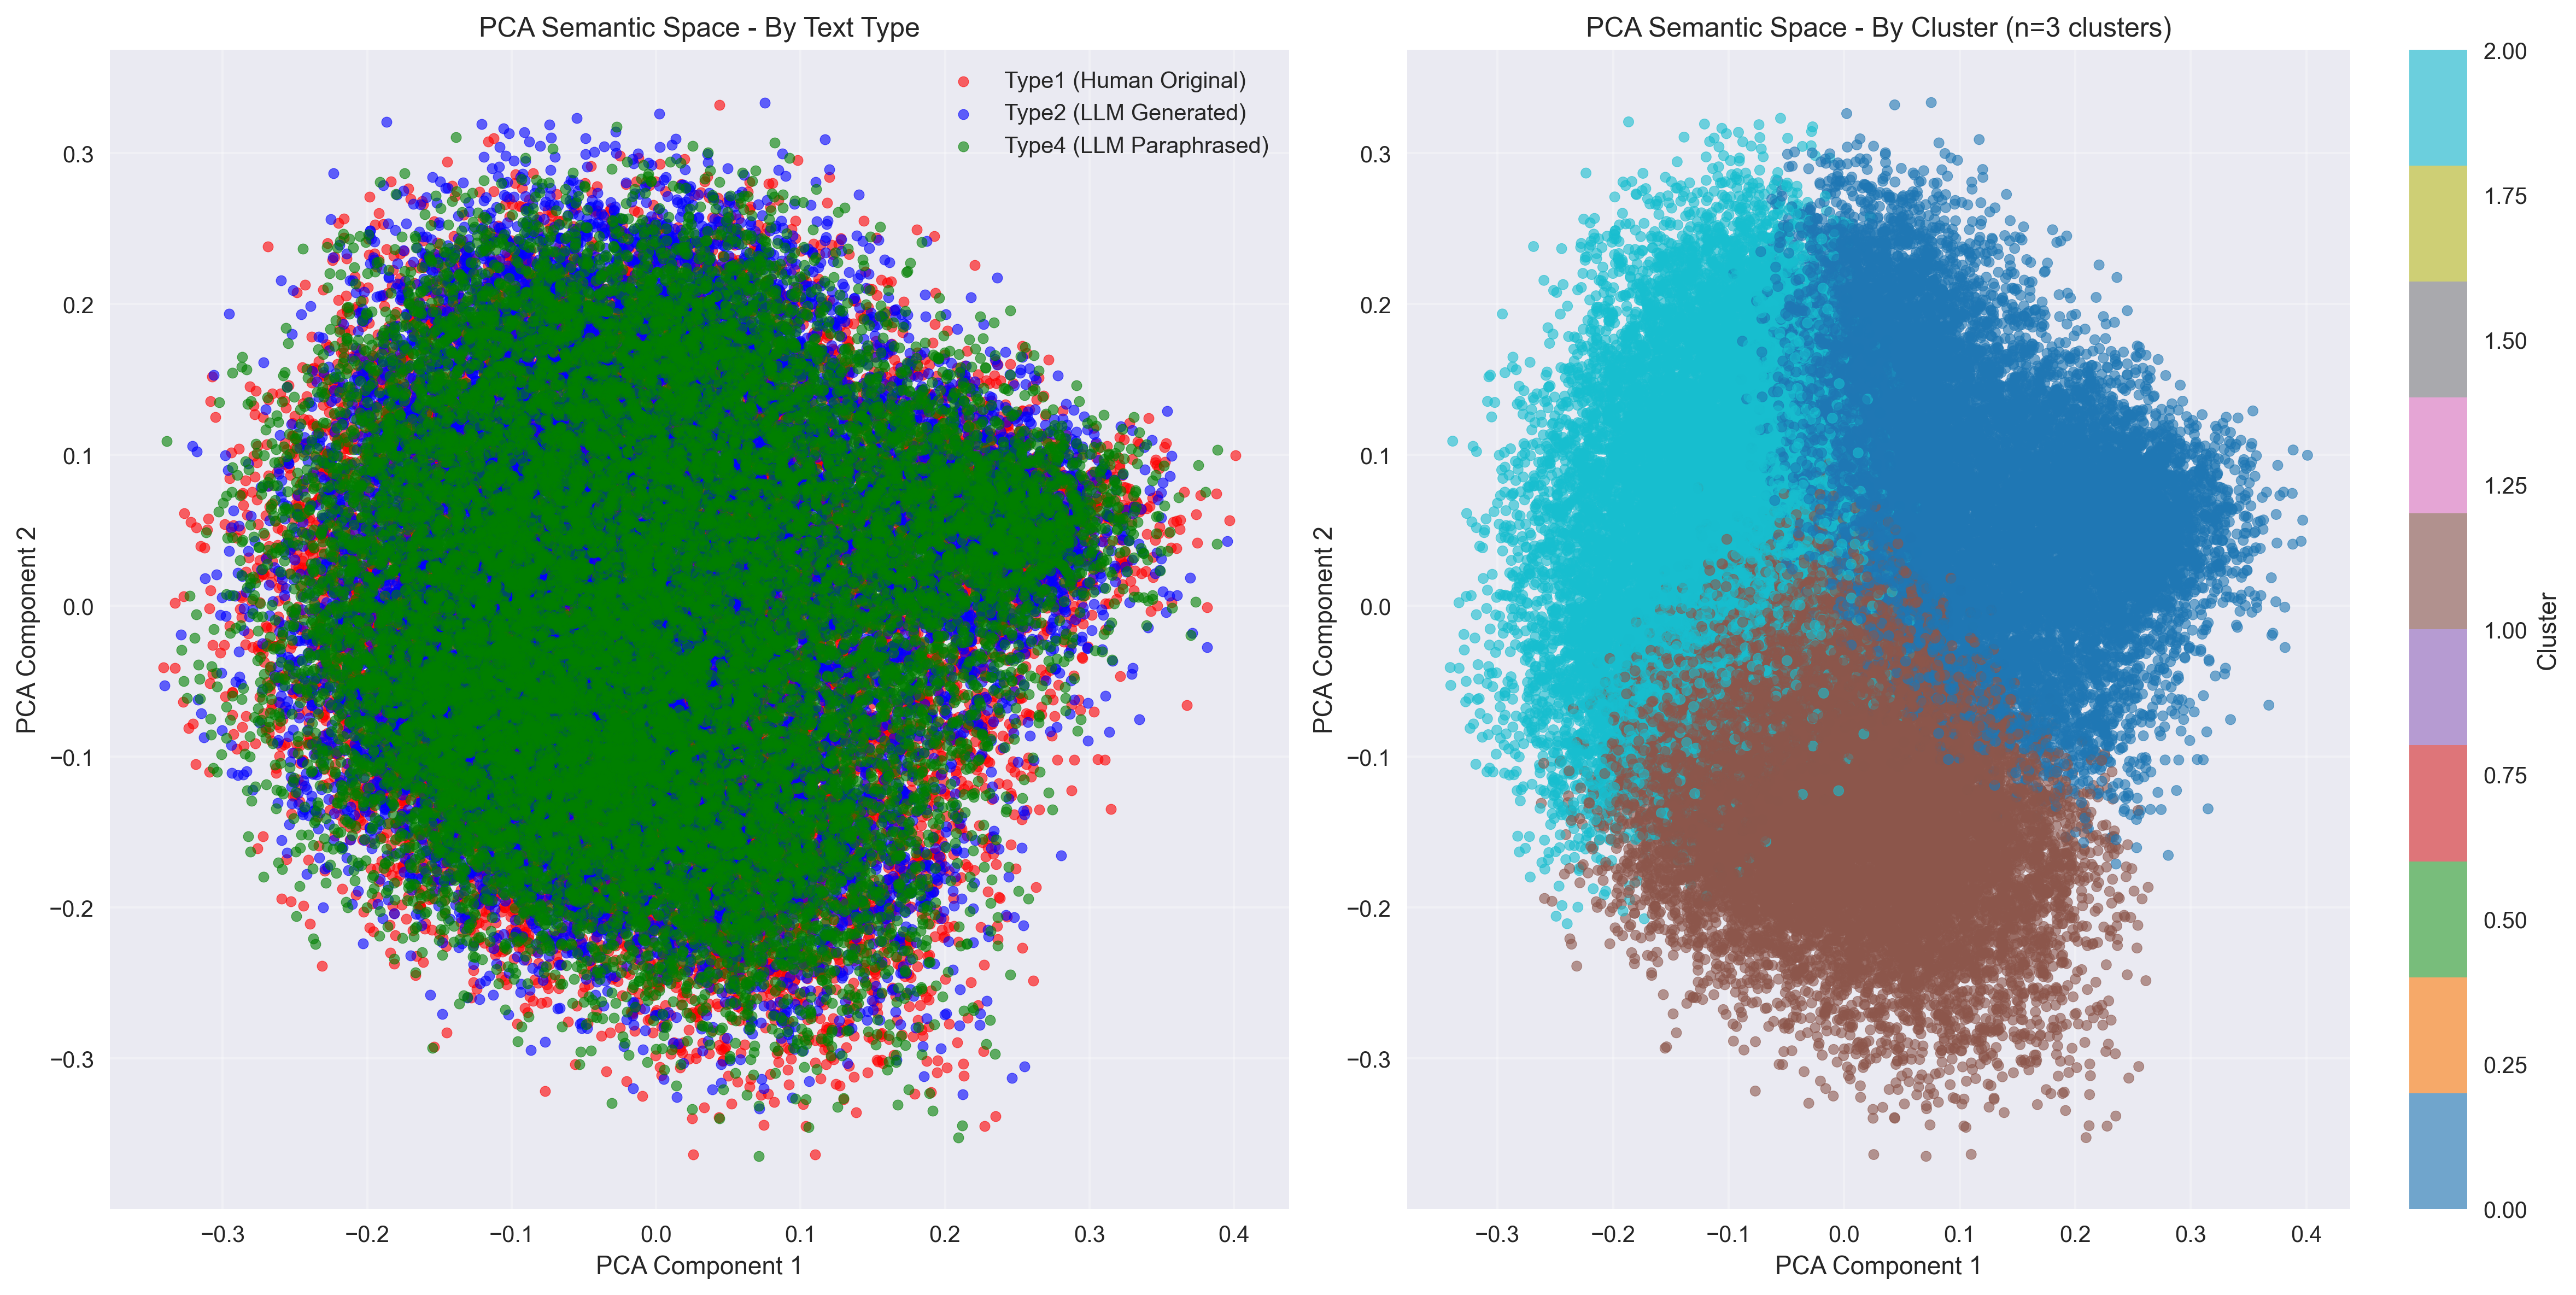
\includegraphics[width=\textwidth]{figures/pca_semantic_space.png}
    \captionof{figure}{PCA projection of semantic space (left) and 
    K-means clustering results (right, $k=3$). Despite measurable 
    distance differences (Table~\ref{tab:pairwise_distances}), text 
    categories show substantial overlap in 2D projection.}
    \label{fig:pca_clustering}
\end{minipage}
\end{figure}
\noindent To reduce the effect of sampling variance, all distance 
measurements are averaged over 5 independent runs. 
Table~\ref{tab:pairwise_distances} (full table is available in \appref{B}) reports the mean pairwise distances 
between the three centroids of the text category. The empirical results yield the following ordering:
\begin{equation}
    \text{dist}\!\left(\bar{\phi}(\mathcal{X}_{\text{para}}),\,
    \bar{\phi}(\mathcal{X}_{\text{human}})\right)
    \;<\;
    \text{dist}\!\left(\bar{\phi}(\mathcal{X}_{\text{human}}),\,
    \bar{\phi}(\mathcal{X}_{\text{gen}})\right)
    \;<\;
    \text{dist}\!\left(\bar{\phi}(\mathcal{X}_{\text{para}}),\,
    \bar{\phi}(\mathcal{X}_{\text{gen}})\right)
    \label{eq:h1_empirical}
\end{equation}
i.e., $0.068 < 0.195 < 0.214$, which 
confirms Hypothesis~\ref{hyp:semantic_displacement}: $\mathcal{X}_{\text{para}}$
constitutes a qualitatively distinct text category.

\noindent An interesting finding emerges from the PCA projection of 
the representation space (Figure~\ref{fig:pca_clustering}): despite 
the clear distance ordering confirmed in Equation~\ref{eq:h1_empirical}, 
all three categories show substantial overlap in 2D PCA space, with 
K-means clustering failing to recover text-type-aligned boundaries. 
This indicates that the discriminative signal between 
$\mathcal{X}_{\text{human}}$, $\mathcal{X}_{\text{gen}}$, and 
$\mathcal{X}_{\text{para}}$ is distributed across many high-dimensional 
directions simultaneously, rather than concentrating along the first 
two principal components. This explains why zero-shot statistical 
detectors---which operate on low-dimensional statistical summaries of 
text---fail to capture the separation between these categories, as we 
confirm empirically in Section~\ref{sec:results}.

%% -------------------------------------------------------
%% HYPOTHESIS 2
%% -------------------------------------------------------
\subsection{Hypothesis 2 Discussion}
\noindent Hypothesis~\ref{hyp:semantic_displacement} establishes that 
$\mathcal{X}_{\text{para}}$ occupies a distinct region in $\phi$-space 
that lies closer to $\mathcal{X}_{\text{human}}$ than to 
$\mathcal{X}_{\text{gen}}$. This raises a natural follow-up question: 
if a single paraphrasing step already moves text toward the human-authored 
region, does \textit{iterative} paraphrasing continue this trajectory, 
progressively making text more human-like and thus increasingly harder 
to detect?

\noindent\textbf{Notation.} Let $x^{(0)} \in \mathcal{X}$ denote an 
original text, and let $x^{(k)} = \text{Para}^{(k)}(x^{(0)})$ denote 
the text after $k$ iterations of LLM paraphrasing, where each iteration 
applies the paraphrasing operation to the output of the previous one. 
For a text set $\mathcal{X}_t$ of origin type $t \in \{\text{human}, 
\text{gen}\}$, the centroid after $k$ iterations is:
\begin{equation}
    \bar{\phi}^{(k)}(\mathcal{X}_t) = \frac{1}{|\mathcal{X}_t|}
    \sum_{x \in \mathcal{X}_t} \phi\!\left(\text{Para}^{(k)}(x)\right)
    \label{eq:iterative_centroid}
\end{equation}
where $\bar{\phi}^{(0)}(\mathcal{X}_t) = \bar{\phi}(\mathcal{X}_t)$ 
denotes the centroid of the original unparaphrased texts.

\begin{hypothesis}
\label{hyp:laundering_convergence}
Iterative paraphrasing progressively moves text toward 
$\mathcal{X}_{\text{human}}$, making it increasingly indistinguishable 
from human-authored content. Specifically, the distance between 
iteratively paraphrased text and $\mathcal{X}_{\text{human}}$ decreases 
monotonically with iteration count $k$:
\begin{equation}
    \text{dist}\!\left(\bar{\phi}^{(k+1)}(\mathcal{X}_t),\,
    \bar{\phi}^{(0)}(\mathcal{X}_{\text{human}})\right)
    \;<\;
    \text{dist}\!\left(\bar{\phi}^{(k)}(\mathcal{X}_t),\,
    \bar{\phi}^{(0)}(\mathcal{X}_{\text{human}})\right)
    \label{eq:h2}
\end{equation}
for both $t \in \{\text{human}, \text{gen}\}$ and all $k \geq 0$. 
\end{hypothesis}

\noindent\textbf{Experiment 2 Setup.} 1000 texts are sampled from each 
of $\mathcal{X}_{\text{human}}$ and $\mathcal{X}_{\text{gen}}$, with 
$k=10$ paraphrasing iterations performed using Qwen3-4B-Instruct, 
yielding iteratively paraphrased sets 
$\{x^{(k)}\}_{k=1}^{10}$ for each origin type. For each iteration, 
the following are extracted: (1)~paraphrased text, (2)~final layer 
hidden states (4096-dim) with mean pooling, and (3)~BGE-M3 embeddings 
(1024-dim). Cosine similarities are computed between iteration centroids 
and reference centroids $\bar{\phi}^{(0)}(\mathcal{X}_{\text{human}})$ 
and $\bar{\phi}^{(0)}(\mathcal{X}_{\text{gen}})$, with PCA applied to 
centroid trajectories (\appref{B}).

\noindent\textbf{Experiment 2 Results.}

\begin{table}[t]
\raggedright
\tiny
\begin{minipage}[c]{0.46\textwidth}
\raggedright
\setlength{\tabcolsep}{2pt}
\captionof{table}{Cosine similarity between iteratively paraphrased text 
and reference centroids $\bar{\phi}^{(0)}(\mathcal{X}_{\text{human}})$ 
and $\bar{\phi}^{(0)}(\mathcal{X}_{\text{gen}})$ in BGE-M3 embedding 
space. Full table in \appref{B}.}
\label{tab:semantic_distances}
\begin{tabular}{@{}llccccc@{}}
\toprule
\multirow{2}{*}{\textbf{Ref.}} & 
\multirow{2}{*}{\textbf{Origin}} &
\multicolumn{5}{c}{\textbf{Iteration} $k$} \\
\cmidrule(lr){3-7}
& & \textbf{2} & \textbf{4} & \textbf{6} & \textbf{8} & \textbf{10} \\
\midrule
\multirow{2}{*}{$\bar{\phi}^{(0)}_{\text{human}}$}
& $\mathcal{X}_{\text{human}}$ & 0.085 & 0.107 & 0.122 & 0.128 & 0.134 \\
& $\mathcal{X}_{\text{gen}}$   & 0.698 & 0.697 & 0.697 & 0.699 & 0.698 \\
\bottomrule
\end{tabular}
\end{minipage}
\hfill
\begin{minipage}[c]{0.50\textwidth}
\raggedright
\setlength{\tabcolsep}{2pt}
\captionsetup{justification=raggedright, singlelinecheck=false}
\captionof{table}{Cosine similarity between consecutive iterations 
$\text{dist}(\bar{\phi}^{(k)}(\mathcal{X}_t), 
\bar{\phi}^{(k+1)}(\mathcal{X}_t))$ for $t \in 
\{\mathcal{X}_{\text{human}}, \mathcal{X}_{\text{gen}}\}$ 
under BGE-M3 embeddings and Qwen3-4B hidden states.}
\label{tab:iterative_distances}
\begin{tabular}{@{}llccccc@{}}
\toprule
\multirow{2}{*}{\textbf{Repr.}} & 
\multirow{2}{*}{\textbf{Origin}} & 
\multicolumn{5}{c}{\textbf{Iteration} $k$} \\
\cmidrule(lr){3-7}
& & \textbf{2} & \textbf{4} & \textbf{6} & \textbf{8} & \textbf{10} \\
\midrule
\multirow{2}{*}{BGE Emb.}
& $\mathcal{X}_{\text{human}}$ & 0.048 & 0.072 & 0.083 & 0.092 & 0.100 \\
& $\mathcal{X}_{\text{gen}}$   & 0.047 & 0.068 & 0.077 & 0.087 & 0.091 \\
\midrule
\multirow{2}{*}{Hid. Stat.}
& $\mathcal{X}_{\text{human}}$ & 0.012 & 0.022 & 0.015 & 0.017 & 0.019 \\
& $\mathcal{X}_{\text{gen}}$   & 0.011 & 0.014 & 0.015 & 0.017 & 0.018 \\
\bottomrule
\end{tabular}
\end{minipage}
\end{table}

\noindent Table~\ref{tab:semantic_distances} directly tests 
Hypothesis~\ref{hyp:laundering_convergence}. For 
$\mathcal{X}_{\text{human}}$, the cosine similarity to 
$\bar{\phi}^{(0)}(\mathcal{X}_{\text{human}})$ increases monotonically 
with $k$ ($0.085 \to 0.134$), and for $\mathcal{X}_{\text{gen}}$, 
the cosine similarity to $\bar{\phi}^{(0)}(\mathcal{X}_{\text{human}})$ remains 
stable ($\approx 0.698$ across all iterations). Both observations 
\textbf{reject Hypothesis~\ref{hyp:laundering_convergence}}---iterative 
paraphrasing does not move text progressively closer to 
$\mathcal{X}_{\text{human}}$; instead it drifts \textit{away} from its 
own origin while maintaining a constant distance from 
$\mathcal{X}_{\text{gen}}$.

\noindent Table~\ref{tab:iterative_distances} further examines the 
inter-iteration drift dynamics 
$\text{dist}(\bar{\phi}^{(k)}(\mathcal{X}_t), \bar{\phi}^{(k+1)}(\mathcal{X}_t))$ 
for $t \in \{\mathcal{X}_{\text{human}}, \mathcal{X}_{\text{gen}}\}$, 
$k \geq 1$, revealing two key patterns.

\noindent\textbf{(1) Decelerating Semantic Drift.} Under BGE-M3 
embeddings, the inter-iteration cosine similarity accumulates for both $\mathcal{X}_{\text{human}}$ ($0.048 \to 0.100$) 
and $\mathcal{X}_{\text{gen}}$ ($0.047 \to 0.091$), confirming 
cumulative semantic displacement with each paraphrasing step. Additionally, the \textit{rate} of displacement decelerates as $k$ 
increases---the gain from iteration 1 to 4 ($0.072$) is substantially 
larger than from iteration 4 to 10 ($0.028$ for 
$\mathcal{X}_{\text{human}}$). This diminishing return indicates that 
beyond a certain depth, additional paraphrasing iterations introduce 
only trivial semantic change while risking incoherence in the generated 
text. This motivates our benchmark design choice to cap at 
1-iteration and 3-iteration variants in PADBen.

\noindent\textbf{(2) Representation-Dependent Drift Magnitude.} 
BGE-M3 embeddings exhibit substantially larger inter-iteration 
displacement ($0.047$--$0.100$) than Qwen3-4B hidden states 
($0.011$--$0.022$). This divergence reflects fundamental differences 
in what each representation captures---BGE-M3's contrastive training 
is optimized to track \textit{semantic content} variations, while 
Qwen3-4B hidden states encode \textit{generation-level patterns} 
(lexical choices, syntactic constructions, stylistic regularities) 
learned during causal language model pre-training. The stability of 
hidden-state distances across iterations therefore provides evidence 
that generation-level patterns are more resistant to paraphrase 
perturbation than semantic content.

\noindent Together, these two patterns lead to a revised understanding: 
rather than moving text toward $\mathcal{X}_{\text{human}}$ as 
Hypothesis~\ref{hyp:laundering_convergence} predicted, iterative 
paraphrasing induces \textit{cumulative semantic drift away from the 
source} while \textit{preserving generation-level patterns}. This 
mechanism enables two distinct attack scenarios. \textbf{(1) Authorship 
Obfuscation:} Human-authored text undergoing iterative paraphrasing 
maintains human-like stylistic markers despite semantic drift, creating 
detection blind spots that enable unauthorized appropriation of human 
writing. \textbf{(2) Plagiarism Evasion:} LLM-generated text 
experiencing iterative paraphrasing preserves AI-like generation 
patterns while achieving sufficient semantic transformation to evade 
plagiarism detection systems, facilitating academic misconduct.

\begin{figure*}[t]
    \centering
    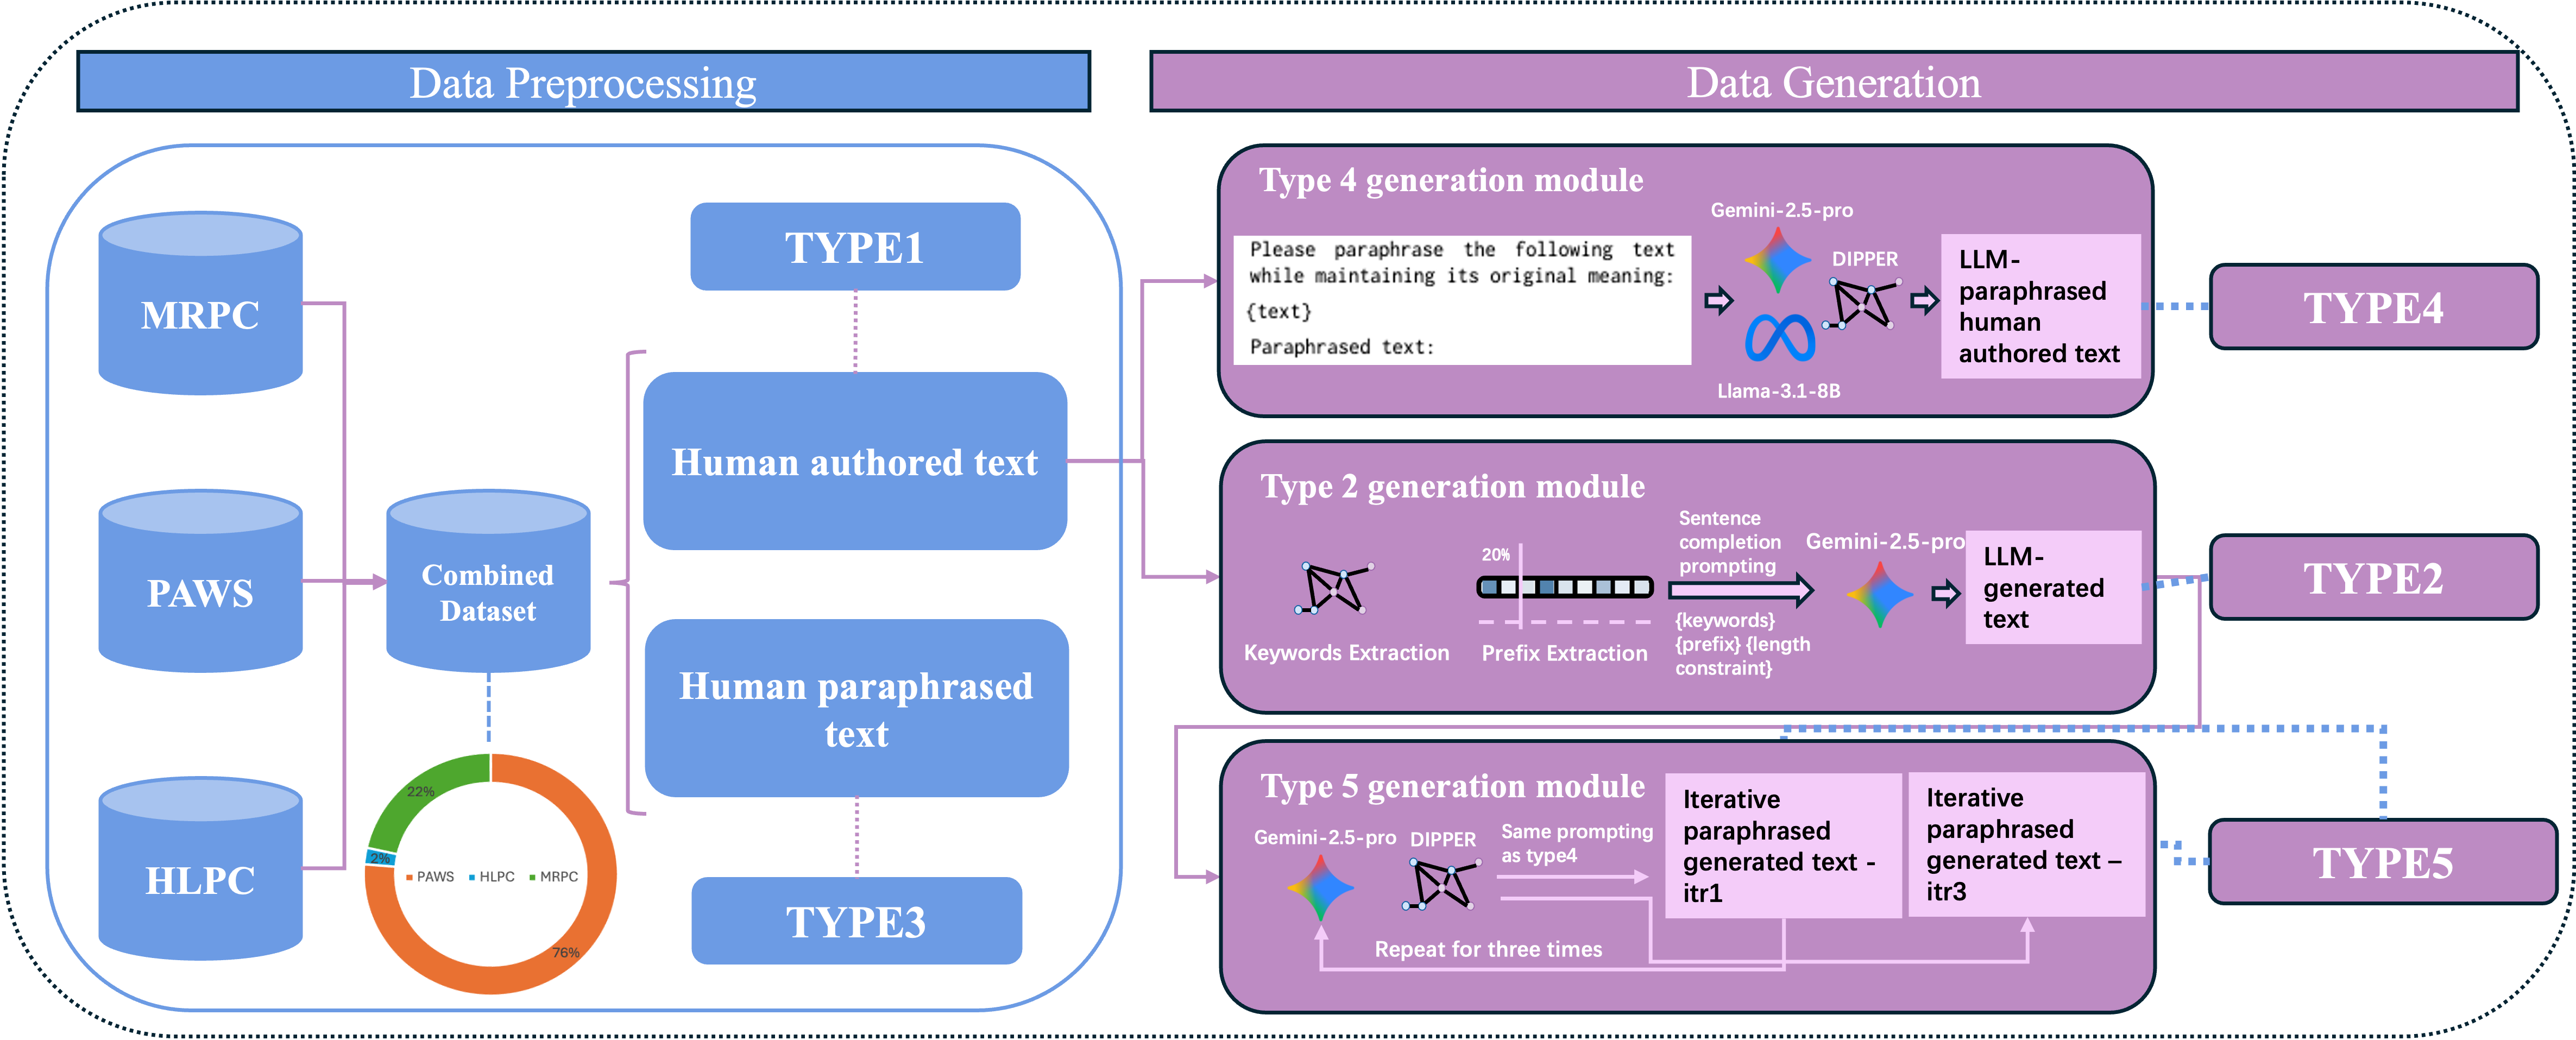
\includegraphics[width=\textwidth]{figures/Overall_pipeline.png}
    \caption{Overall pipeline for benchmark curation. Preprocessing 
    details in \appref{A}, data generation in 
    \appref{C}.}
    \label{fig:overall_pipeline}
\end{figure*}

\begin{figure*}[t]
    \centering
     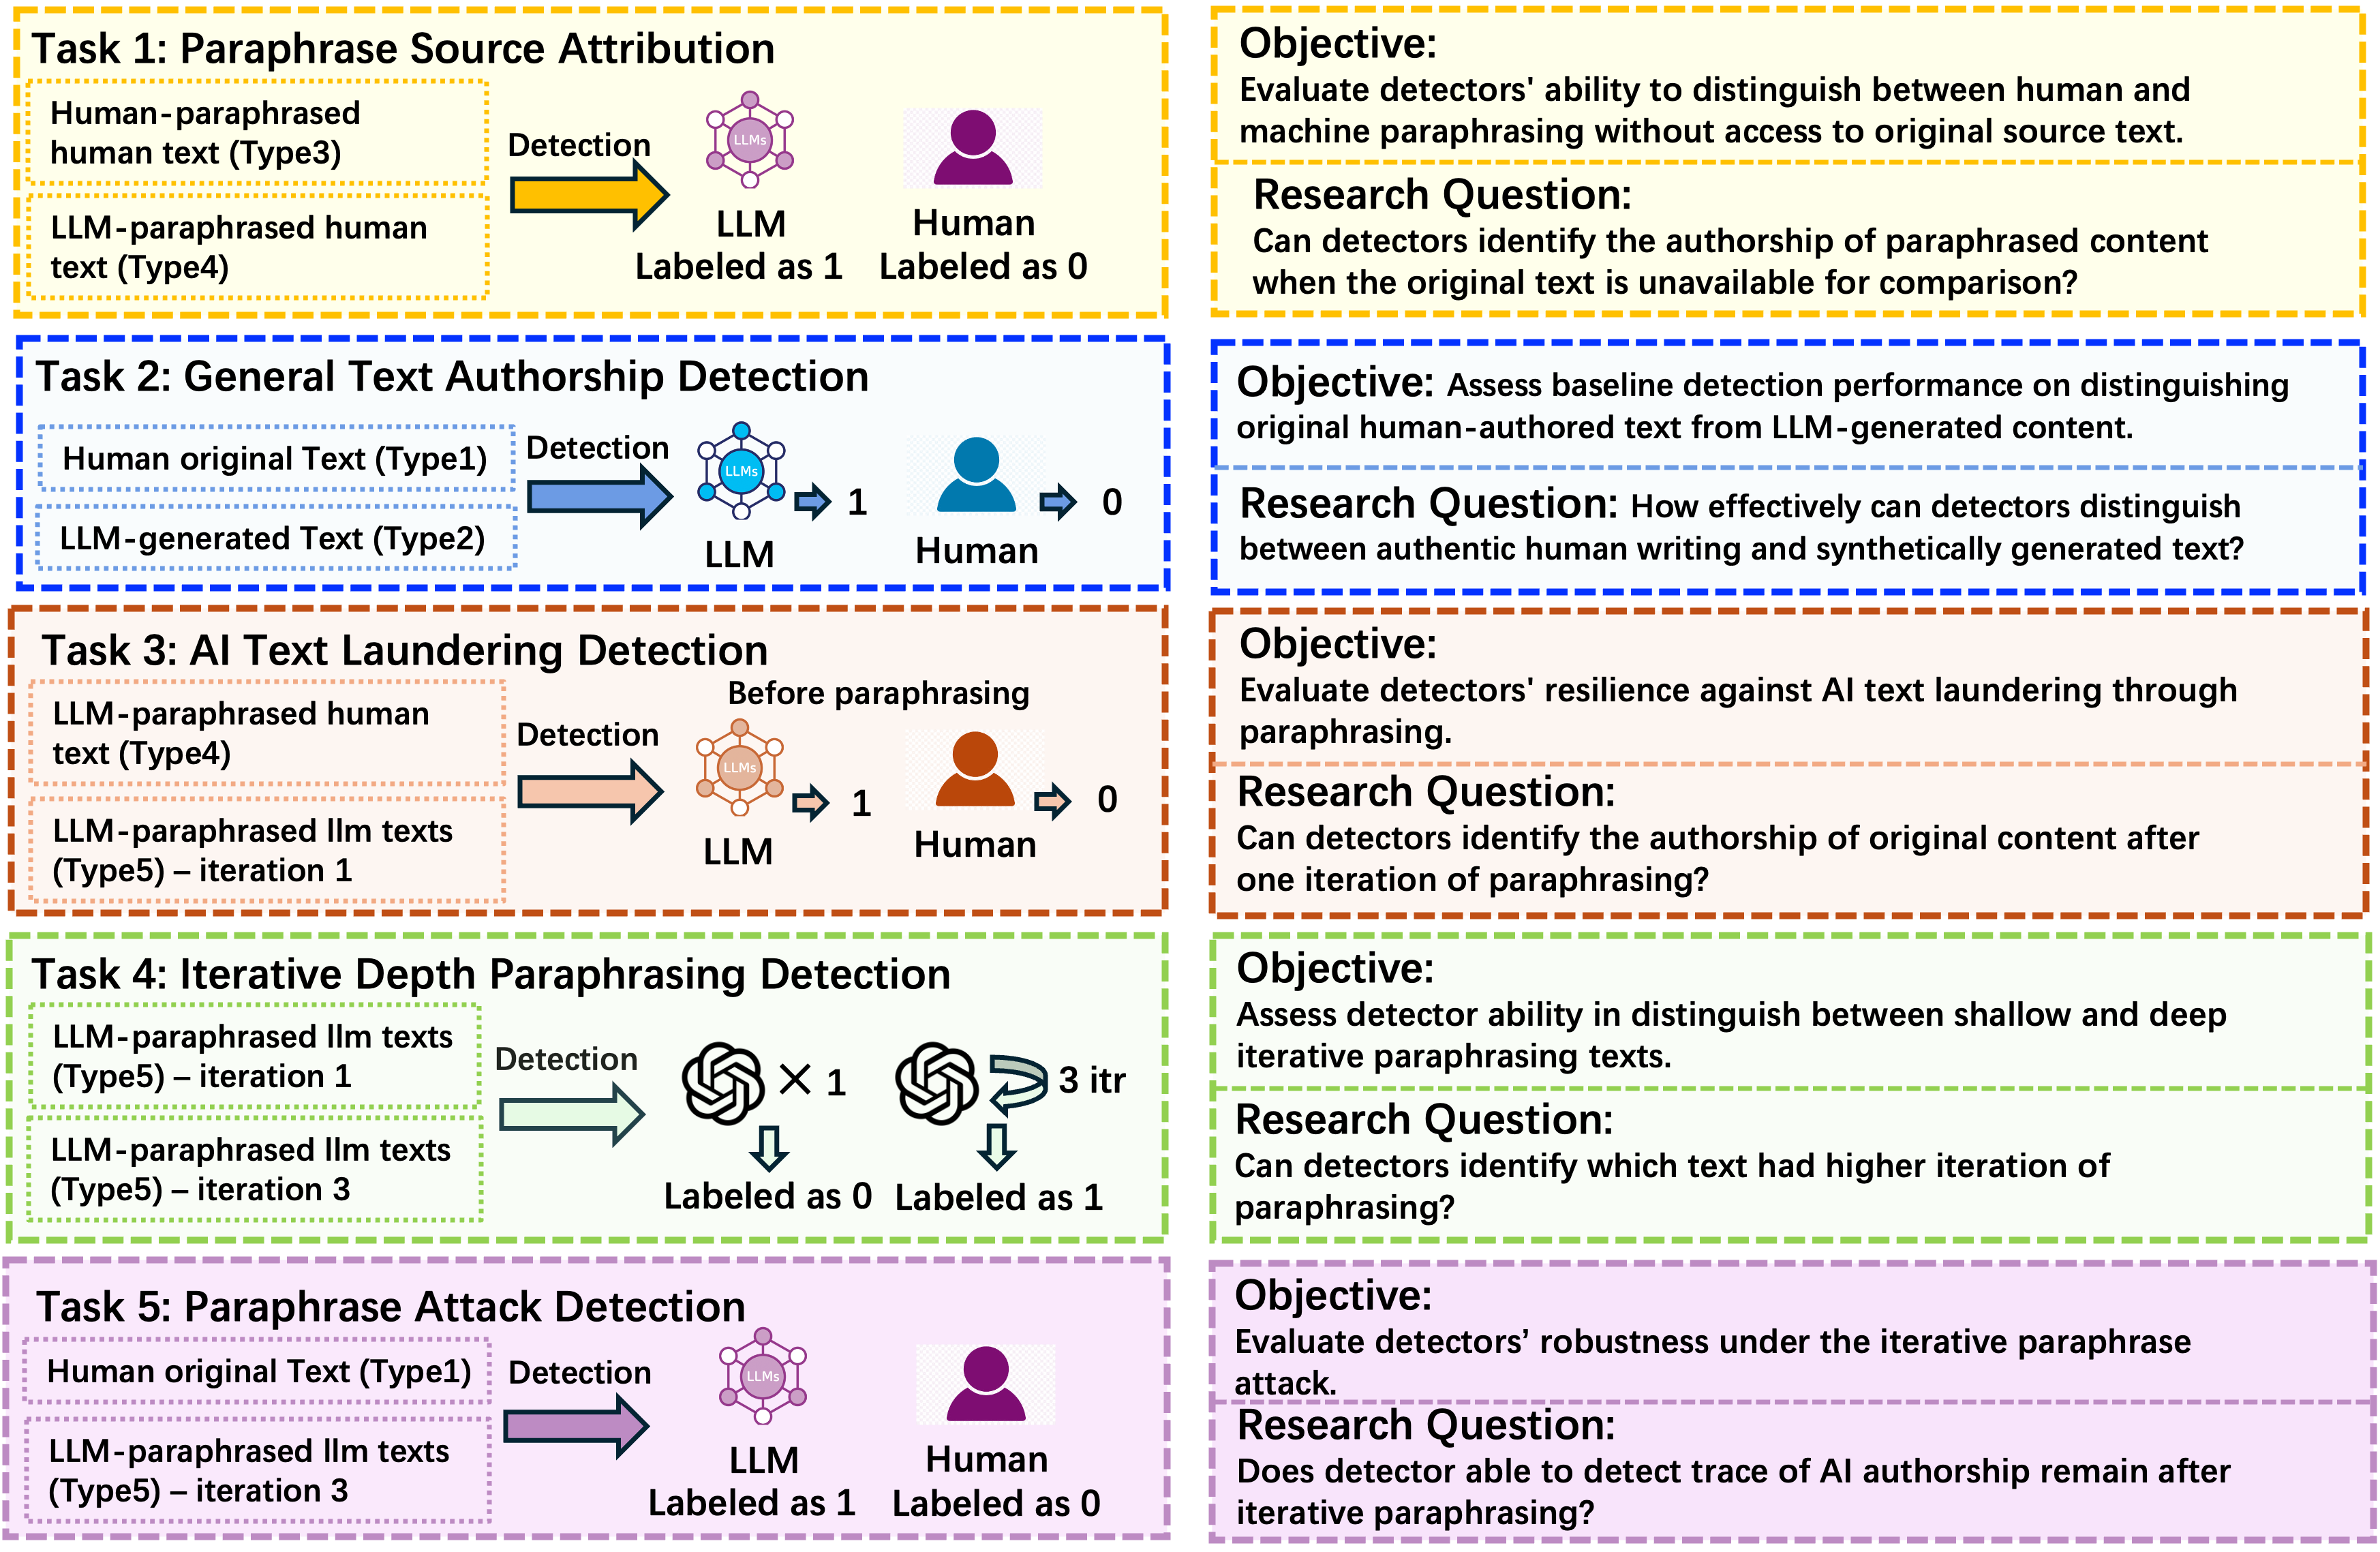
\includegraphics[width=\textwidth]{figures/task_intro.png}
    \caption{Overall Task introduction for the Benchmark. Task 1-5 measures the detector's different capabilities covering the robustness, performance when encountering the paraphrase attack. Detailed task specifics can be found in \appref{C}.}
    \label{fig:task_intro}
\end{figure*}


\section{Benchmark Curation}

\noindent\textbf{Text Type Taxonomy.}
\noindent The two attack scenarios identified in Section~\ref{sec:mechanism} 
map onto distinct real-world threats: (a)~\textit{Authorship obfuscation}: 
a writer paraphrases human-authored text through an LLM to evade 
stylometric attribution or plagiarism detection---the paraphrase must 
appear human-authored. (b)~\textit{Plagiarism evasion}: an author 
paraphrases LLM-generated content iteratively to remove detectable AI 
artifacts before submission---the output must evade AIGT classifiers. 
These two scenarios require fundamentally different text collections to 
evaluate: the former compares human paraphrases (Type 3) vs.\ LLM 
paraphrases (Type 4) of human text; the latter contrasts deeply laundered 
AI text (Type 5) against baselines (Types 1, 2). The taxonomy is therefore 
grounded in these two threat scenarios and is not ad-hoc. A five-category 
taxonomy is established: \textbf{Type 1} --- Human original text; 
\textbf{Type 2} --- LLM-generated text; \textbf{Type 3} --- 
Human-paraphrased human text; \textbf{Type 4} --- LLM-paraphrased human 
text; \textbf{Type 5} --- LLM-iteratively-paraphrased LLM text. Detailed 
definitions can be found in \appref{C}.

\noindent\textbf{Data Preparation.}
The benchmark leverages three established datasets: Microsoft Research 
Paraphrase Corpus (\textbf{MRPC})~\cite{dolan2005automatically}, 
Human-LLM Paraphrase Corpus (\textbf{HLPC})~\cite{lau2024hlpc}, and 
Paraphrase Adversaries from Word Scrambling 
(\textbf{PAWS})~\cite{paws2019naacl}. A cosine similarity filter 
(threshold: 0.85) is applied to remove near-duplicates, combining them 
to obtain 16,233 human-authored texts (Type 1) and human-paraphrased 
human texts (Type 3). Figure~\ref{fig:overall_pipeline} illustrates 
the detailed procedure of how raw data is preprocessed and how Type 2, 
4, and 5 texts are generated via a modularized generation pipeline: 
\textbf{Type 2} via sentence completion using Google Gemini-2.5-Pro; 
\textbf{Type 4} via multi-model paraphrasing (DIPPER, Gemini-2.5-Pro, 
LLaMA-3-8B); and \textbf{Type 5} via iterative paraphrasing with 
temperature scaling and convergence detection.

\noindent\textbf{Quality Assurance.}
Dataset quality is verified using three metrics: Jaccard 
similarity (inter-type semantic preservation), perplexity (linguistic 
diversity), and self-BLEU (intra-type diversity). Full analysis, 
including comparison with the RAID benchmark, is provided in 
\appref{C}. PADBen achieves substantially higher 
diversity and perplexity than RAID.

\noindent\textbf{Task Introduction.}
Five progressive detection tasks are designed to systematically assess 
detector's robustness in varying complexity levels and attack 
scenarios. Each task targets specific vulnerabilities while leveraging 
the multi-type text dataset to evaluate detectors under increasingly 
sophisticated adversarial conditions. Figure~\ref{fig:task_intro} 
demonstrates the description of the five tasks, and 
\appref{C} provides further details on task 
objectives.


\begin{table}[t]
\centering
\caption{Zero-shot Detectors Performance Summary}
\label{tab:appendix_zero_shot_complete}
\small
\setlength{\tabcolsep}{3pt}
\resizebox{\textwidth}{!}{%
\begin{tabular}{lll|cccc|cccc|cccc|cccc|cccc}
\toprule
\textbf{MODEL} & \textbf{CHALLENGE} & \textbf{METHOD}
& \multicolumn{4}{c|}{\textbf{Task 1}}
& \multicolumn{4}{c|}{\textbf{Task 2}}
& \multicolumn{4}{c|}{\textbf{Task 3}}
& \multicolumn{4}{c|}{\textbf{Task 4}}
& \multicolumn{4}{c}{\textbf{Task 5}} \\
 & & & AUC & T1 & T5 & T10 & AUC & T1 & T5 & T10 & AUC & T1 & T5 & T10 & AUC & T1 & T5 & T10 & AUC & T1 & T5 & T10 \\
\midrule
\multirow{5}{*}{BINOCULAR}
 & sentence-pair   &      & 0.399 & 0.003 & 0.023 & 0.050 & 0.457 & 0.007 & 0.037 & 0.081 & 0.505 & 0.008 & 0.046 & 0.099 & 0.498 & \underline{\textcolor{blue}{0.011}} & 0.052 & 0.106 & 0.457 & 0.006 & 0.032 & 0.070 \\
 & single-sentence & exhaustive     & 0.439 & \underline{\textcolor{blue}{0.011}} & \underline{\textcolor{blue}{0.046}} & 0.080 & 0.579 & \underline{\textcolor{blue}{0.029}} & \underline{\textcolor{blue}{0.106}} & \underline{\textcolor{blue}{0.184}} & 0.500 & 0.008 & 0.050 & 0.101 & 0.486 & \underline{\textcolor{blue}{0.012}} & 0.050 & 0.098 & 0.428 & 0.009 & \underline{\textcolor{blue}{0.047}} & 0.087 \\
 & single-sentence & sampling\_30\% & 0.437 & \underline{\textcolor{blue}{0.010}} & \underline{\textcolor{blue}{0.046}} & 0.081 & 0.575 & \underline{\textcolor{blue}{0.031}} & \underline{\textcolor{blue}{0.109}} & \underline{\textcolor{blue}{0.188}} & 0.495 & 0.008 & 0.050 & 0.096 & 0.486 & \underline{\textcolor{blue}{0.010}} & \underline{\textcolor{blue}{0.051}} & 0.098 & 0.429 & 0.008 & \underline{\textcolor{blue}{0.050}} & 0.090 \\
 & single-sentence & sampling\_50\% & 0.443 & \underline{\textcolor{blue}{0.011}} & \underline{\textcolor{blue}{0.047}} & 0.084 & 0.583 & \underline{\textcolor{blue}{0.032}} & \underline{\textcolor{blue}{0.112}} & \underline{\textcolor{blue}{0.194}} & 0.499 & 0.008 & 0.051 & 0.102 & 0.487 & \underline{\textcolor{blue}{0.012}} & \underline{\textcolor{blue}{0.053}} & 0.099 & 0.434 & 0.009 & \underline{\textcolor{blue}{0.051}} & 0.092 \\
 & single-sentence & sampling\_80\% & 0.453 & \underline{\textcolor{blue}{0.010}} & \underline{\textcolor{blue}{0.049}} & 0.087 & 0.589 & \underline{\textcolor{blue}{0.034}} & \underline{\textcolor{blue}{0.116}} & \underline{\textcolor{blue}{0.195}} & 0.507 & 0.007 & 0.058 & 0.106 & 0.487 & \textbf{\textcolor{red}{0.016}} & \textbf{\textcolor{red}{0.060}} & \underline{\textcolor{blue}{0.104}} & 0.439 & \underline{\textcolor{blue}{0.012}} & \underline{\textcolor{blue}{0.053}} & 0.092 \\
\midrule
\multirow{5}{*}{\begin{tabular}{@{}l@{}}FAST\_DETECT\\\_GPT\end{tabular}}
 & sentence-pair   &      & \underline{\textcolor{blue}{0.638}} & \textbf{\textcolor{red}{0.027}} & \textbf{\textcolor{red}{0.115}} & \underline{\textcolor{blue}{0.204}} & \underline{\textcolor{blue}{0.787}} & \underline{\textcolor{blue}{0.086}} & \underline{\textcolor{blue}{0.249}} & \underline{\textcolor{blue}{0.369}} & 0.503 & \underline{\textcolor{blue}{0.012}} & 0.055 & 0.108 & 0.476 & 0.005 & 0.036 & 0.081 & \underline{\textcolor{blue}{0.606}} & 0.023 & \underline{\textcolor{blue}{0.090}} & \underline{\textcolor{blue}{0.165}} \\
 & single-sentence & exhaustive     & \underline{\textcolor{blue}{0.573}} & 0.006 & 0.044 & \underline{\textcolor{blue}{0.099}} & \underline{\textcolor{blue}{0.665}} & 0.010 & 0.075 & 0.149 & 0.504 & 0.011 & 0.051 & 0.103 & 0.488 & 0.009 & 0.051 & 0.099 & \underline{\textcolor{blue}{0.568}} & 0.006 & 0.047 & \underline{\textcolor{blue}{0.103}} \\
 & single-sentence & sampling\_30\% & \underline{\textcolor{blue}{0.576}} & 0.006 & \underline{\textcolor{blue}{0.046}} & \underline{\textcolor{blue}{0.097}} & \underline{\textcolor{blue}{0.666}} & 0.009 & 0.078 & 0.154 & 0.502 & 0.011 & 0.049 & 0.096 & 0.490 & 0.007 & 0.046 & 0.091 & \underline{\textcolor{blue}{0.572}} & 0.005 & 0.045 & \underline{\textcolor{blue}{0.100}} \\
 & single-sentence & sampling\_50\% & \underline{\textcolor{blue}{0.581}} & 0.005 & 0.045 & \underline{\textcolor{blue}{0.098}} & \underline{\textcolor{blue}{0.672}} & 0.010 & 0.078 & 0.153 & 0.505 & 0.010 & 0.051 & 0.101 & 0.491 & 0.008 & 0.049 & 0.095 & \underline{\textcolor{blue}{0.577}} & 0.005 & 0.047 & \underline{\textcolor{blue}{0.102}} \\
 & single-sentence & sampling\_80\% & \underline{\textcolor{blue}{0.587}} & 0.004 & 0.040 & \underline{\textcolor{blue}{0.092}} & \underline{\textcolor{blue}{0.675}} & 0.008 & 0.076 & 0.151 & 0.514 & 0.007 & 0.045 & 0.100 & 0.488 & 0.011 & 0.049 & 0.095 & \underline{\textcolor{blue}{0.578}} & 0.005 & 0.048 & \underline{\textcolor{blue}{0.103}} \\
\midrule
\multirow{5}{*}{GLTR}
 & sentence-pair   &      & 0.429 & \underline{\textcolor{blue}{0.007}} & 0.043 & 0.082 & 0.436 & 0.006 & 0.045 & 0.086 & \underline{\textcolor{blue}{0.529}} & 0.011 & \underline{\textcolor{blue}{0.060}} & \underline{\textcolor{blue}{0.116}} & \underline{\textcolor{blue}{0.514}} & \textbf{\textcolor{red}{0.016}} & \textbf{\textcolor{red}{0.057}} & \textbf{\textcolor{red}{0.113}} & 0.482 & \underline{\textcolor{blue}{0.012}} & 0.054 & 0.108 \\
 & single-sentence & exhaustive     & 0.459 & 0.006 & 0.032 & 0.068 & 0.480 & 0.004 & 0.021 & 0.056 & \underline{\textcolor{blue}{0.513}} & \underline{\textcolor{blue}{0.012}} & \underline{\textcolor{blue}{0.059}} & \underline{\textcolor{blue}{0.122}} & \underline{\textcolor{blue}{0.506}} & \textbf{\textcolor{red}{0.013}} & \textbf{\textcolor{red}{0.057}} & \textbf{\textcolor{red}{0.113}} & 0.488 & \underline{\textcolor{blue}{0.011}} & 0.047 & 0.091 \\
 & single-sentence & sampling\_30\% & 0.457 & 0.004 & 0.034 & 0.066 & 0.474 & 0.003 & 0.019 & 0.053 & \underline{\textcolor{blue}{0.519}} & \underline{\textcolor{blue}{0.012}} & \underline{\textcolor{blue}{0.065}} & \underline{\textcolor{blue}{0.124}} & \underline{\textcolor{blue}{0.502}} & \textbf{\textcolor{red}{0.014}} & \textbf{\textcolor{red}{0.056}} & \textbf{\textcolor{red}{0.109}} & 0.484 & \underline{\textcolor{blue}{0.012}} & 0.045 & 0.085 \\
 & single-sentence & sampling\_50\% & 0.461 & 0.005 & 0.036 & 0.068 & 0.480 & 0.004 & 0.022 & 0.057 & \underline{\textcolor{blue}{0.524}} & \underline{\textcolor{blue}{0.012}} & \underline{\textcolor{blue}{0.066}} & \underline{\textcolor{blue}{0.126}} & \textbf{\textcolor{red}{0.507}} & \textbf{\textcolor{red}{0.015}} & \textbf{\textcolor{red}{0.059}} & \textbf{\textcolor{red}{0.114}} & 0.489 & \underline{\textcolor{blue}{0.011}} & 0.049 & 0.089 \\
 & single-sentence & sampling\_80\% & 0.458 & 0.006 & 0.031 & 0.063 & 0.482 & 0.004 & 0.021 & 0.059 & \underline{\textcolor{blue}{0.523}} & \underline{\textcolor{blue}{0.011}} & \underline{\textcolor{blue}{0.062}} & \underline{\textcolor{blue}{0.117}} & \textbf{\textcolor{red}{0.509}} & \underline{\textcolor{blue}{0.013}} & \underline{\textcolor{blue}{0.059}} & \textbf{\textcolor{red}{0.111}} & 0.491 & 0.011 & 0.047 & 0.095 \\
\midrule
\multirow{5}{*}{RADAR}
 & sentence-pair   &      & \textbf{\textcolor{red}{0.728}} & 0.004 & \underline{\textcolor{blue}{0.105}} & \textbf{\textcolor{red}{0.246}} & \textbf{\textcolor{red}{0.910}} & \textbf{\textcolor{red}{0.142}} & \textbf{\textcolor{red}{0.566}} & \textbf{\textcolor{red}{0.809}} & \textbf{\textcolor{red}{0.748}} & \textbf{\textcolor{red}{0.054}} & \textbf{\textcolor{red}{0.234}} & \textbf{\textcolor{red}{0.372}} & \textbf{\textcolor{red}{0.526}} & 0.010 & \underline{\textcolor{blue}{0.055}} & \underline{\textcolor{blue}{0.112}} & \textbf{\textcolor{red}{0.909}} & \textbf{\textcolor{red}{0.140}} & \textbf{\textcolor{red}{0.542}} & \textbf{\textcolor{red}{0.808}} \\
 & single-sentence & exhaustive     & \textbf{\textcolor{red}{0.648}} & \textbf{\textcolor{red}{0.038}} & \textbf{\textcolor{red}{0.190}} & \textbf{\textcolor{red}{0.345}} & \textbf{\textcolor{red}{0.793}} & \textbf{\textcolor{red}{0.063}} & \textbf{\textcolor{red}{0.313}} & \textbf{\textcolor{red}{0.567}} & \textbf{\textcolor{red}{0.633}} & \textbf{\textcolor{red}{0.016}} & \textbf{\textcolor{red}{0.080}} & \textbf{\textcolor{red}{0.160}} & \textbf{\textcolor{red}{0.511}} & 0.010 & \underline{\textcolor{blue}{0.052}} & \underline{\textcolor{blue}{0.104}} & \textbf{\textcolor{red}{0.797}} & \textbf{\textcolor{red}{0.062}} & \textbf{\textcolor{red}{0.310}} & \textbf{\textcolor{red}{0.562}} \\
 & single-sentence & sampling\_30\% & \textbf{\textcolor{red}{0.642}} & \textbf{\textcolor{red}{0.037}} & \textbf{\textcolor{red}{0.187}} & \textbf{\textcolor{red}{0.337}} & \textbf{\textcolor{red}{0.789}} & \textbf{\textcolor{red}{0.063}} & \textbf{\textcolor{red}{0.313}} & \textbf{\textcolor{red}{0.560}} & \textbf{\textcolor{red}{0.627}} & \textbf{\textcolor{red}{0.016}} & \textbf{\textcolor{red}{0.078}} & \textbf{\textcolor{red}{0.157}} & \textbf{\textcolor{red}{0.508}} & \underline{\textcolor{blue}{0.010}} & \underline{\textcolor{blue}{0.051}} & \underline{\textcolor{blue}{0.103}} & \textbf{\textcolor{red}{0.797}} & \textbf{\textcolor{red}{0.062}} & \textbf{\textcolor{red}{0.312}} & \textbf{\textcolor{red}{0.560}} \\
 & single-sentence & sampling\_50\% & \textbf{\textcolor{red}{0.644}} & \textbf{\textcolor{red}{0.036}} & \textbf{\textcolor{red}{0.181}} & \textbf{\textcolor{red}{0.337}} & \textbf{\textcolor{red}{0.789}} & \textbf{\textcolor{red}{0.060}} & \textbf{\textcolor{red}{0.302}} & \textbf{\textcolor{red}{0.559}} & \textbf{\textcolor{red}{0.628}} & \textbf{\textcolor{red}{0.016}} & \textbf{\textcolor{red}{0.078}} & \textbf{\textcolor{red}{0.155}} & \underline{\textcolor{blue}{0.506}} & 0.010 & 0.051 & \underline{\textcolor{blue}{0.102}} & \textbf{\textcolor{red}{0.795}} & \textbf{\textcolor{red}{0.060}} & \textbf{\textcolor{red}{0.300}} & \textbf{\textcolor{red}{0.556}} \\
 & single-sentence & sampling\_80\% & \textbf{\textcolor{red}{0.648}} & \textbf{\textcolor{red}{0.039}} & \textbf{\textcolor{red}{0.195}} & \textbf{\textcolor{red}{0.345}} & \textbf{\textcolor{red}{0.797}} & \textbf{\textcolor{red}{0.067}} & \textbf{\textcolor{red}{0.335}} & \textbf{\textcolor{red}{0.569}} & \textbf{\textcolor{red}{0.630}} & \textbf{\textcolor{red}{0.016}} & \textbf{\textcolor{red}{0.078}} & \textbf{\textcolor{red}{0.156}} & \underline{\textcolor{blue}{0.508}} & 0.010 & 0.051 & 0.102 & \textbf{\textcolor{red}{0.803}} & \textbf{\textcolor{red}{0.066}} & \textbf{\textcolor{red}{0.332}} & \textbf{\textcolor{red}{0.568}} \\
\bottomrule
\end{tabular}%
}
{\raggedright\small\textbf{Note:} AUC = AUC-ROC, T1 = TPR@1\%FPR, T5 = TPR@5\%FPR, T10 = TPR@10\%FPR. Best ({\color{red}\textbf{red bold}}) and second-best ({\color{blue}\underline{blue underlined}}) results are marked within each setup for each task and metric.\par}
\end{table}
\section{Evaluation Framework}
Two categories of detectors are examined: \textbf{1. Zero-shot detectors} 
Operating without task-specific training, relying on pre-existing 
linguistic/statistical patterns to distinguish human vs.\ machine text; 
the evaluated detectors include Binoculars, Fast-Detect-GPT, GLTR, and 
RADAR (\appref{E}). \textbf{2. Model-based 
detectors} Leveraging pre-trained language models or instruction-based 
LLMs for classification, using few-shot and persona prompting strategies 
for both evaluation challenges 
(\appref{E}).

\noindent\textbf{Evaluation Setup.}
Evaluation is conducted under two challenges---single-sentence 
classification and sentence-pair recognition---across 5 setups to 
reflect realistic use cases (\appref{D}): (1)~\textbf{Single-Sentence 
Exhaustive}: all samples with balanced 50-50 distribution; \\
(2)~\textbf{Sampling (30-70)}: 30\% positive, 70\% negative; \\
(3)~\textbf{Sampling (50-50)}: balanced random sampling; \\
(4)~\textbf{Sampling (80-20)}: 80\% positive, 20\% negative; \\
(5)~\textbf{Sentence-Pair Recognition}: pairwise comparison with 
random order presentation. \\
Full implementation details are provided 
in \appref{D}.


\begin{table}[t]
\centering
\caption{Model-based Detectors Performance Summary}
\label{tab:appendix_model_based_complete}
\small
\setlength{\tabcolsep}{3pt}
\resizebox{\textwidth}{!}{%
\begin{tabular}{ll|cccc|cccc|cccc|cccc|cccc}
\toprule
\textbf{Model} & \textbf{Challenge}
& \multicolumn{4}{c|}{\textbf{Task 1}}
& \multicolumn{4}{c|}{\textbf{Task 2}}
& \multicolumn{4}{c|}{\textbf{Task 3}}
& \multicolumn{4}{c|}{\textbf{Task 4}}
& \multicolumn{4}{c}{\textbf{Task 5}} \\
 &  & \textbf{AUC} & \textbf{T1} & \textbf{T5} & \textbf{T10}
      & \textbf{AUC} & \textbf{T1} & \textbf{T5} & \textbf{T10}
      & \textbf{AUC} & \textbf{T1} & \textbf{T5} & \textbf{T10}
      & \textbf{AUC} & \textbf{T1} & \textbf{T5} & \textbf{T10}
      & \textbf{AUC} & \textbf{T1} & \textbf{T5} & \textbf{T10} \\
\midrule
\multirow{2}{*}{Claude-3.5-Haiku}
& sentence-pair
& \underline{\textcolor{blue}{0.623}} & \underline{\textcolor{blue}{0.016}} & \underline{\textcolor{blue}{0.078}} & \underline{\textcolor{blue}{0.155}} & 0.366 & 0.005 & 0.024 & 0.047 & 0.475 & \underline{\textcolor{blue}{0.010}} & 0.042 & 0.085 & 0.507 & \underline{\textcolor{blue}{0.010}} & 0.051 & 0.102 & 0.351 & 0.003 & 0.017 & 0.034 \\
& single-sentence
& \textbf{\textcolor{red}{0.514}} & \textbf{\textcolor{red}{0.012}} & \underline{\textcolor{blue}{0.058}} & \textbf{\textcolor{red}{0.115}} & \underline{\textcolor{blue}{0.535}} & \textbf{\textcolor{red}{0.018}} & \textbf{\textcolor{red}{0.089}} & \textbf{\textcolor{red}{0.162}} & 0.519 & \underline{\textcolor{blue}{0.022}} & \underline{\textcolor{blue}{0.069}} & 0.069 & 0.503 & \underline{\textcolor{blue}{0.011}} & 0.054 & 0.073 & \underline{\textcolor{blue}{0.545}} & \textbf{\textcolor{red}{0.049}} & \underline{\textcolor{blue}{0.112}} & \underline{\textcolor{blue}{0.112}} \\
\midrule
\multirow{2}{*}{DeepSeek-V2.5}
& sentence-pair
& 0.572 & 0.012 & 0.060 & 0.120 & 0.467 & 0.008 & 0.039 & 0.078 & \textbf{\textcolor{red}{0.519}} & \textbf{\textcolor{red}{0.011}} & \textbf{\textcolor{red}{0.057}} & \textbf{\textcolor{red}{0.113}} & \textbf{\textcolor{red}{0.514}} & \textbf{\textcolor{red}{0.011}} & \textbf{\textcolor{red}{0.054}} & \textbf{\textcolor{red}{0.108}} & 0.484 & 0.009 & 0.046 & 0.091 \\
& single-sentence
& 0.480 & 0.009 & 0.046 & 0.092 & 0.479 & 0.009 & 0.047 & 0.095 & \underline{\textcolor{blue}{0.531}} & 0.014 & \underline{\textcolor{blue}{0.069}} & \textbf{\textcolor{red}{0.138}} & 0.501 & 0.010 & 0.051 & 0.101 & 0.511 & 0.011 & 0.055 & 0.110 \\
\midrule
\multirow{2}{*}{Gemma-3-27B}
& sentence-pair
& 0.521 & 0.011 & 0.053 & 0.105 & \underline{\textcolor{blue}{0.506}} & \underline{\textcolor{blue}{0.010}} & 0.051 & \underline{\textcolor{blue}{0.102}} & 0.480 & \underline{\textcolor{blue}{0.010}} & 0.048 & 0.095 & 0.502 & \underline{\textcolor{blue}{0.010}} & 0.050 & 0.101 & 0.516 & \underline{\textcolor{blue}{0.010}} & 0.052 & 0.104 \\
& single-sentence
& 0.461 & 0.008 & 0.040 & 0.080 & 0.465 & 0.009 & 0.044 & 0.088 & 0.520 & 0.013 & 0.064 & 0.129 & 0.503 & 0.010 & 0.052 & 0.104 & 0.478 & 0.009 & 0.043 & 0.085 \\
\midrule
\multirow{2}{*}{Kimi-K2-Instruct}
& sentence-pair
& \textbf{\textcolor{red}{0.691}} & \textbf{\textcolor{red}{0.020}} & \textbf{\textcolor{red}{0.102}} & \textbf{\textcolor{red}{0.204}} & 0.431 & 0.007 & 0.036 & 0.071 & \underline{\textcolor{blue}{0.516}} & \textbf{\textcolor{red}{0.011}} & 0.053 & 0.106 & 0.487 & \underline{\textcolor{blue}{0.010}} & 0.048 & 0.096 & 0.441 & 0.006 & 0.030 & 0.060 \\
& single-sentence
& \underline{\textcolor{blue}{0.509}} & \textbf{\textcolor{red}{0.012}} & \textbf{\textcolor{red}{0.062}} & 0.096 & \textbf{\textcolor{red}{0.540}} & \underline{\textcolor{blue}{0.014}} & \underline{\textcolor{blue}{0.071}} & \underline{\textcolor{blue}{0.141}} & \textbf{\textcolor{red}{0.540}} & \textbf{\textcolor{red}{0.029}} & \textbf{\textcolor{red}{0.123}} & 0.123 & 0.503 & \underline{\textcolor{blue}{0.011}} & \textbf{\textcolor{red}{0.056}} & 0.063 & \textbf{\textcolor{red}{0.573}} & \underline{\textcolor{blue}{0.047}} & \textbf{\textcolor{red}{0.185}} & \textbf{\textcolor{red}{0.185}} \\
\midrule
\multirow{2}{*}{\begin{tabular}{@{}l@{}}Llama-4-Scout\\-17B\end{tabular}}
& sentence-pair
& 0.561 & 0.012 & 0.059 & 0.118 & 0.456 & 0.008 & 0.042 & 0.085 & \textbf{\textcolor{red}{0.519}} & \textbf{\textcolor{red}{0.011}} & \underline{\textcolor{blue}{0.054}} & \underline{\textcolor{blue}{0.109}} & 0.493 & \underline{\textcolor{blue}{0.010}} & 0.049 & 0.098 & 0.476 & 0.009 & 0.046 & 0.091 \\
& single-sentence
& 0.486 & 0.009 & 0.047 & 0.095 & 0.472 & 0.009 & 0.046 & 0.091 & 0.523 & 0.013 & 0.065 & \underline{\textcolor{blue}{0.131}} & \textbf{\textcolor{red}{0.509}} & \underline{\textcolor{blue}{0.011}} & \underline{\textcolor{blue}{0.055}} & \textbf{\textcolor{red}{0.111}} & 0.506 & 0.010 & 0.052 & 0.103 \\
\midrule
\multirow{2}{*}{Mistral-Nemo}
& sentence-pair
& 0.510 & 0.014 & 0.069 & 0.073 & 0.504 & \textbf{\textcolor{red}{0.011}} & \textbf{\textcolor{red}{0.057}} & 0.066 & 0.501 & \underline{\textcolor{blue}{0.010}} & 0.051 & 0.101 & 0.502 & \underline{\textcolor{blue}{0.010}} & 0.051 & 0.101 & \underline{\textcolor{blue}{0.518}} & \textbf{\textcolor{red}{0.012}} & \underline{\textcolor{blue}{0.059}} & \underline{\textcolor{blue}{0.118}} \\
& single-sentence
& 0.489 & 0.009 & 0.044 & 0.089 & 0.470 & 0.008 & 0.040 & 0.081 & 0.494 & 0.008 & 0.038 & 0.040 & 0.493 & 0.009 & 0.046 & 0.091 & 0.498 & 0.009 & 0.046 & 0.049 \\
\midrule
\multirow{2}{*}{\begin{tabular}{@{}l@{}}WizardLM-2\\-8x22B\end{tabular}}
& sentence-pair
& 0.558 & 0.012 & 0.059 & 0.119 & \textbf{\textcolor{red}{0.520}} & \textbf{\textcolor{red}{0.011}} & \underline{\textcolor{blue}{0.054}} & \textbf{\textcolor{red}{0.108}} & 0.508 & \underline{\textcolor{blue}{0.010}} & \underline{\textcolor{blue}{0.052}} & 0.103 & \underline{\textcolor{blue}{0.510}} & \underline{\textcolor{blue}{0.010}} & \underline{\textcolor{blue}{0.052}} & \underline{\textcolor{blue}{0.104}} & \textbf{\textcolor{red}{0.551}} & \textbf{\textcolor{red}{0.012}} & \textbf{\textcolor{red}{0.061}} & \textbf{\textcolor{red}{0.122}} \\
& single-sentence
& 0.501 & \underline{\textcolor{blue}{0.010}} & 0.050 & \underline{\textcolor{blue}{0.101}} & 0.505 & 0.011 & 0.053 & 0.105 & 0.505 & 0.013 & 0.045 & 0.045 & \underline{\textcolor{blue}{0.504}} & \textbf{\textcolor{red}{0.012}} & 0.049 & 0.049 & 0.499 & 0.009 & 0.047 & 0.048 \\
\bottomrule
\end{tabular}%
}
{\raggedright\small\textbf{Note:} AUC = AUC-ROC, T1 = TPR@1\%FPR, T5 = TPR@5\%FPR, T10 = TPR@10\%FPR. Single-sentence evaluation uses 50--50 sampling. Best ({\color{red}\textbf{red bold}}) and second-best ({\color{blue}\underline{blue underlined}}) results are marked within each setup for each task and metric.\par}
\end{table}

\section{Results}
\label{sec:results}
Tables~\ref{tab:appendix_zero_shot_complete} and 
\ref{tab:appendix_model_based_complete} report complete results across 
4 zero-shot and 7 model-based detectors across five tasks and evaluation setups. 

\noindent\textbf{Task 1 (Paraphrase Source Attribution).}
Both detector categories struggle with absolute classification (AUC 
0.46--0.52 single-sentence). RADAR achieves the best results (AUC 
0.728 sentence-pair, 0.648 exhaustive), followed by Kimi-K2-Instruct 
(AUC 0.691 sentence-pair). The improved sentence-pair performance 
suggests that comparative signals partially compensate for the 
difficulty of distinguishing human paraphrases (Type 3) from LLM 
paraphrases (Type 4) in isolation.

\noindent\textbf{Task 2 (General Authorship Detection).}
RADAR dominates with AUC 0.910 (sentence-pair) and 0.797 (exhaustive). 
Model-based detectors underperform substantially (best: Kimi AUC 0.540 
single-sentence), suggesting instruction-following LLMs cannot exploit 
representation-space differences between $\mathcal{X}_{\text{human}}$ 
and $\mathcal{X}_{\text{gen}}$ without task-specific fine-tuning.

\noindent\textbf{Task 3 (AI Text Laundering Detection).}
Performance degrades substantially across most detectors. RADAR 
maintains moderate sentence-pair capability (AUC 0.748), but this 
represents a 16-point drop from its Task 2 performance---consistent 
with the authorship obfuscation blind spot identified in 
Section~\ref{sec:mechanism}. Single-sentence performance collapses 
to near-random across all detectors (AUC 0.47--0.54), confirming that 
once texts undergo iterative paraphrasing, source origin becomes 
unreliable for absolute classification.

\noindent\textbf{Task 4 (Iterative Depth Detection).}
Near-random performance across all detectors (AUC 0.487--0.529). 
Rather than a detector failure per se, this is a fundamental 
consequence of the small semantic difference between 1-iteration and 
3-iteration paraphrasing identified in Section~\ref{sec:mechanism}. 
Task 4 serves as a deliberate stress test probing the detection floor, 
motivating future depth-aware detection methods.

\noindent\textbf{Task 5 (Paraphrase Attack Detection).}
RADAR demonstrates strong performance (AUC 0.909 sentence-pair, 0.803 
exhaustive), confirming that deeply laundered AI text preserves 
detectable generation artifacts against $\mathcal{X}_{\text{human}}$ 
baselines. Model-based detectors show modest capability (best: Kimi 
AUC 0.573 single-sentence) but cannot match RADAR's fine-tuned 
sensitivity to generation-level patterns.

\noindent\textbf{Common Observations.}

\noindent\textit{Two Attack Categories Empirically Confirmed.} 
Task 3's difficulty (best AUC 0.748; near-random for most detectors) 
versus Task 5's tractability (best AUC 0.909) empirically validates 
the asymmetry predicted by the mechanistic analysis: both tasks involve 
iteratively paraphrased text, but authorship obfuscation (Task 3) 
erases the source signal while plagiarism evasion (Task 5) preserves 
detectable generation artifacts. The gap between these two tasks is 
the central empirical finding of PADBen.

\noindent\textit{Representation Space Asymmetry.} RADAR's consistent 
superiority across Tasks 2, 3, and 5 reflects its adversarial training 
on generation-level patterns that instruction-following models cannot 
access through prompting alone---confirming that generation-level 
features require task-specific fine-tuning to exploit.

\noindent\textit{Evaluation Robustness.} Single-sentence sampling 
variants show stable performance (variation $\leq 0.02$ AUC across 
all splits), confirming results reflect stylistic discrimination rather 
than base-rate exploitation. Zero-shot detectors consistently benefit 
from sentence-pair evaluation ($+0.1$--$0.2$ AUC), while model-based 
detectors show inconsistent patterns attributable to nondeterministic 
generation.

\section{Conclusion}

This paper presents PADBen, the first benchmark to systematically 
evaluate AI text detectors against iterative paraphrase attacks across 
two distinct scenarios: authorship obfuscation and plagiarism evasion. Evaluation of 11 detectors across five tasks confirms the predicted 
asymmetry: plagiarism evasion remains detectable (RADAR AUC 0.909) 
while authorship obfuscation substantially degrades all detectors 
(best AUC 0.748, near-random for most). These findings demonstrate 
that current binary human-vs-AIGT classifiers still lack robustness when facing the paraphrase attack setting, motivating detection 
methods that go beyond binary semantic and stylistic discrimination. The mechanism analysis relies on BGE-M3 embeddings and Qwen3-4B 
hidden states; quantitative replication with other models and direct 
measurement of lexical/syntactic feature stability are reserved for 
future work. Extending PADBen to deeper iteration depths and additional 
paraphrasing models would further characterize the detection floor 
identified in Task 4.

\bibliographystyle{unsrt}
\bibliography{padben}
\begin{credits}
\subsubsection{\discintname}
The authors have no competing interests to declare that are relevant to the content of this article.
\end{credits}

\end{document}
